\documentclass[parskip=full]{scrartcl}
\usepackage{geometry}
\geometry{a4paper, left=2.5cm, right=2cm, top=3cm, bottom=3cm}
\usepackage[utf8]{inputenc} % use utf8 file encoding for TeX sources
\usepackage[T1]{fontenc}    % avoid garbled Unicode text in pdf
\usepackage[german]{babel}  % german hyphenation, quotes, etc
\usepackage{hyperref}       % detailed hyperlink/pdf configuration
\hypersetup{                % ‘texdoc hyperref‘ for options
pdftitle={Echtzeit-Computergrafik in der Spieleentwicklung},%
bookmarks=true,
}

\usepackage{rotating}
\usepackage{newclude}
\usepackage{typearea}
\newcommand\invisiblesection[1]{%
  \refstepcounter{section}%
  \addcontentsline{toc}{section}{\protect\numberline{\thesection}#1}%
  \sectionmark{#1}}


\usepackage{listings}

\usepackage{xcolor}
\usepackage{graphicx}       % provides commands for including figures
\usepackage{csquotes}       % provides \enquote{} macro for "quotes"
\usepackage[nonumberlist]{glossaries}     % provides glossary commands
\usepackage{enumitem}
\usepackage{epsf,epsfig,eepic}
\usepackage[headsepline, footsepline]{scrpage2}


%Design für Methoden-/Attributbeschreibungen
\usepackage{framed}
\usepackage{color}
\definecolor{gray}{RGB}{200,200,200}
\renewenvironment{leftbar}[1][\hsize]
{%
\def\FrameCommand
{%
{\color{gray}\vrule width 1pt}%     
}%
\MakeFramed{\hsize#1\advance\hsize-\width\FrameRestore}%
}
{\endMakeFramed}

\definecolor{eclipseStrings}{HTML}{B71C1C}
\definecolor{eclipseKeywords}{HTML}{0D47A1}
\definecolor{background}{HTML}{ECEFF1}
\colorlet{numb}{magenta!60!black}

\lstdefinelanguage{json}{
    basicstyle=\normalfont\ttfamily,
    commentstyle=\color{eclipseStrings}, % style of comment
    stringstyle=\color{eclipseKeywords}, % style of strings
    numbers=left,
    numberstyle=\scriptsize,
    stepnumber=1,
    numbersep=8pt,
    showstringspaces=false,
    breaklines=true,
    frame=lines,
    backgroundcolor=\color{background}, %only if you like
    string=[s]{"}{"},
    comment=[l]{:\ "},
    morecomment=[l]{:"},
    literate=
        *{0}{{{\color{numb}0}}}{1}
         {1}{{{\color{numb}1}}}{1}
         {2}{{{\color{numb}2}}}{1}
         {3}{{{\color{numb}3}}}{1}
         {4}{{{\color{numb}4}}}{1}
         {5}{{{\color{numb}5}}}{1}
         {6}{{{\color{numb}6}}}{1}
         {7}{{{\color{numb}7}}}{1}
         {8}{{{\color{numb}8}}}{1}
         {9}{{{\color{numb}9}}}{1}
}

%kopf und fusszeilen
\pagestyle{scrheadings}
\clearscrheadfoot

%kopfzeile
\ihead{\codename}
\ohead{\headmark}
\automark{section}

%fusszeile
\ofoot{\pagemark}
\ifoot{\codename}

\makenoidxglossaries
%
% % Glossareinträge
%

%Kommandos
\newcommand{\codename}{Valaris}


\title{Implementierungsdokument}
\author{Sidney Hansen, Jonas Heinle, Frederik Lingg, Lukas Schölch, Artur Wesner}

\begin{document}

	\begin{titlepage}
		\centering
		{\scshape\LARGE Implementierungsdokument\par}
		\vspace{1cm}
		{\scshape\Large Echtzeit Computergrafik in der Spieleentwicklung \par}
		\vspace{1cm}
		{\huge\bfseries \codename \par}
		\vspace{1cm}
		\includegraphics[width=.5\linewidth]{./Bilder/valaris_t_4096.png}
		\par
		{\vspace{1cm}}
		{\Large\itshape Autoren \\}
		{\Large\itshape Sidney Hansen, Jonas Heinle,\\}
		{\Large\itshape Frederik Lingg, Lukas Schölch, Artur Wesner\par}
		
		\vfill
		Projektbetreuer\par
		Alisa Jung \& Tobias Rapp
		
		\vfill
		
		% Bottom of the page
		{\large \today\par}
	\end{titlepage}

	\tableofcontents 
	\pagebreak
	
	
	\pagebreak
	
	\section{Einleitung}

	Für die Implementierung von Valaris wurde die Gliederung, welche bereits im Pflichtenheft und Entwurf eingehalten wurde,
	weiterhin verwendet. Somit wurden die Module InGame-Grafik, InGame-Interface, Assets, Generierung und GUI zunächst unabhängig voneinander implementiert
	und später zusammen gefügt.
	
	Jedoch wurde aufgrund von ungleichem Arbeitsumfang der Module die Arbeitsaufteilung der Module weniger streng gehalten.
	Zusätzlich ging Zeit verloren, da das zusammenführen der einzelnen Module zum Teil länger dauerte als ursprünglich vorgesehen.
	Ausserdem wurde die Implementierung der Schnittstelle zum anderen Team mehrfach überarbeitet, um komplexität im Simulationsthread zu verringern.
	Die Implementierung der Shader für Physik basierte Materialien erwies sich ebenfalls als komplizierter als gedacht, da es häufig zu Rechenfehlern
	aufgrund der Ungenauigkeit von Gleitkomma-Zahlen kam.

	Das Resultat der Implementierung ist nun eine Anwendung, welche die gesammte Menüführung besitzt, Strecken generieren und vorführen kann.
	Die eigentliche Simulation des Spiels wurde bisher nicht eingegliedert.

	Im Folgenden wird im Detail erleutert, welche Kriterien umgesetzt, welche Aspekte des Entwurfs geändert und welche Unit-Tests verwendet wurden.
	Das Dokument schließt mit dem Vergleich des geplanten und dem tatsächlichen Ablauf der Implementierung anhand von Gantt-Diagrammen ab.

	\pagebreak

	\section{Features}
	\subsection{InGame - Grafik}
\subsubsection{Musskriterien}

\paragraph{Implementiert}
\begin{itemize}
    \item Darstellung physikalisch akkurater Materialien
    \item Darstellung metallener bzw. dielektrischer Materialien
		\item Rendern von undurchsichtigen Objekten
		\item Viele dynamische Lichtquellen gleichzeitig verarbeiten
		\item Schatten von dynamischen Lichtquellen
		\item Effekte
		\begin{itemize}
            \item verschiedene Partikeleffekte (z.B. Explosionen)
        \end{itemize}
        \item Frei fliegende Kamera zum Ansehen der Strecke
\end{itemize}

\subsubsection{Wunschkriterien}

\paragraph{Implementiert}
\begin{itemize}
    \item Animationen an Fahrzeug
    \begin{itemize}
        \item Animieren der Düsen des Fahrzeuges
    \end{itemize}
    \item Leuchtende Oberflächen
\end{itemize}

\paragraph{Nicht Implementiert}
\begin{itemize}
    \item Postprocessing (z.B. MotionBlur)
	\item Animationen an Spielfigur und Fahrzeug
    \begin{itemize}
	\item Klauen der Energie am vorderen Fahrzeug
	\end{itemize}
	\item Verschiedene Fahrzeuge
    \item HDR
	\item FXAA
	\item Soundeffekte
\end{itemize}
	\pagebreak
	\subsection{InGame - Interface}
Im Pflichtenheft wurden zu diesem Modul keine speziellen Anforderungen genannt, daher
werden im Folgenden alle Implementierten-Features als Musskriterien gewertet.

\subsubsection{Musskriterien}
\paragraph{Implementiert}
\begin{itemize}
    \item Übergabe der Daten in voneinander unabhängigen Paketen
    \item Minimale warte Zeiten bei der Übergabe der Pakete
    \item Dynamische Anzahl von Spiel-Objekten in der Szene
    \item Dynamische Anzahl von Eigenschaften eines einzelnen Spiel-Objekts
    \item Übergabe von Spiel-Events (zum Beispiel ende des Rennens) durch das Interface

    \item Eigenschaften für Position, Ranking, Energielevel, Camera, Türstatus, Geschwindigkeit

    \item Laden der Modelle für Spiel-Objekte
    \item Interpretieren der Eigenschaften der SpielObjekte zur korrekten Darstellung in der Szene
\end{itemize}

\paragraph{Nicht Implementiert}
Aufgrund mangelnder Definition von Anforderungen an das Interface gibt es hier keine nicht implementierten
Musskriterien
	\pagebreak
	\subsection{Assets}
\subsubsection{Musskriterien}

\paragraph{Implementiert}
\begin{itemize}
    \item VerbindungsTunnel der Raumstation
    \item Dekorationen für Raumstationselemente
    \item Kuppeln mit planetarischer Umgebing
    \item Hover-Cart
\end{itemize}

\paragraph{Nicht Implementiert}
\begin{itemize}
    \item Energie-Kugeln auf Hover-Cart
    \item Fahrer für Hover-Cart
\end{itemize}

\subsubsection{Wunschkriterien}

\paragraph{Nicht Implementiert}
\begin{itemize}
    \item Verschiedene Verbindungstunnel-Typen
    \item Verschiedene Fahrzeug-Modelle
    \item Animationen für Fahrer
\end{itemize}
	\pagebreak
	\subsection{Generierung}
\subsubsection{Musskriterien}

\paragraph{Implementiert}
\begin{itemize}
    \item Zusammenhängende Strecke mit Start und Ziel
    \item Checkpoints in sinnvollen Abständen
    \item Generierung von unterschiedlichen Streckenführungen
    \item Deterministisch vom Seed abhängig
    \item Keine unbefahrbaren Streckenabschnitte
    \item Definieren von Extremparametern (Bsp. Steigung, Schärfe der Kurven, ...)
    \item Konform zum Streckenmodell des anderen Teams
    \item (Generierung von Streckenumgebung)
\end{itemize}

\paragraph{Nicht Implementiert}
\begin{itemize}
    \item Assets als Streckenumgebung in Kuppeln
\end{itemize}

\subsubsection{Wunschkriterien}

\paragraph{Implementiert}
\begin{itemize}
    \item Verschiedene Biome
		
\end{itemize}

\paragraph{Nicht Implementiert}
\begin{itemize}
    \item Verschiedene befahrbare Untergründe
	\item Einfügen von Hindernissen auf die Rennbahn
    \item Dynamische Strecken- bzw. Umgebungselemente
\end{itemize}
	\pagebreak
	\subsection{GUI}
\subsubsection{Musskriterien}

\paragraph{Implementiert}
\begin{itemize}
    \item Allgemeines Start-Menü
	\item Einstellungsfenster
    \begin{itemize}
        \item Diverse Möglichkeiten zur Konfiguration des Spielverhaltens
        \item Diverse Möglichkeiten zur Konfiguration der Grafik
    \end{itemize}
    \item Vor dem Spiel:
    \begin{itemize}
        \item Konfiguration des Seed
        \item Auswählen eines gespeicherten Seed
        \item Definition der Anzahl an optionaler KI
    \end{itemize}
    \item Ein während des Spiels aufrufbares Pause-Menü mit den Funktionen:
    \begin{itemize}
        \item Zurückkehren zum Spiel
        \item Zurückkehren zum Start-Menü
        \item Öffnen der Einstellungen
        \item Speichern des aktuellen Seed
    \end{itemize}
    \item Nach dem Spiel:
    \begin{itemize}
        \item Möglichkeit zur Speicherung des aktuellen Seed
        \item Eine Ergebnisanzeige mit Visualisierung der Endposition und der gefahrenen Zeit eines jeden Spielers
        \item Möglichkeit die Strecke erneut zu fahren
        \item Zurückkehren zum Start-Menü
    \end{itemize}
    \pagebreak
    \item Anzeige eines Head-up-Displays(HUD) während dem Spiel
    \begin{itemize}
        \item Aktuell gefahrene Zeit
        \item Visualisierung des aufgesammelten Powerups
        \item Anzeige der aktuellen Ranglistenplatzierung
    \end{itemize}
\end{itemize}

\paragraph{Nicht Implementiert}
\begin{itemize}
    \item Vor dem Spiel:
    \begin{itemize}
        \item Auswählen des Spielmodus
    \end{itemize}
    \item Anzeige eines Head-up-Displays(HUD) während dem Spiel
    \begin{itemize}
        \item Mini-Map in 2D inklusive Visualisierung der Fahrer
        \item Anzeige der Rundenzahl
        \item Anzeige der Geschwindigkeit des Fahrers
    \end{itemize}
\end{itemize}

\subsubsection{Wunschkriterien}

\paragraph{Implementiert}

\paragraph{Nicht Implementiert}
\begin{itemize}
    \item Konfigurationseinstellung für den Ton
    \item Fahrzeugauswahl
    \item Beispielvorschau eines Seed
    \item Abstimmmöglichkeit unter Spielern, ob eine Strecke erneut gespielt werden soll
\end{itemize}
	\pagebreak

	\section{Änderungen}
	\subsection{InGame - Grafik}

\subsubsection{Partikel}
\begin{itemize}
    \item \textit{Darstellung eines Partikels}
        \begin{leftbar}[0.9\linewidth]
            Partikel hat nun einen Transform, der Rotation, Translation, Größe
            des Partikels bündelt.
        \end{leftbar}
\end{itemize}

\subsubsection{Shader und MaterialDef}
\begin{itemize}
    \item \textit{Wechsel der BRDF}
        \begin{leftbar}[0.9\linewidth]
            Disney's principled BRDF hat an Kanten kleine weiße Pixel produziert.
            Wechsel zum Ansatz, der die Unreal Engine macht, um Problem zu umgehen.
        \end{leftbar}
\end{itemize}

\subsubsection{PartikelEffekt}
\begin{itemize}
    \item \textit{Farbe als Vertexattribut}
        \begin{leftbar}[0.9\linewidth]
        Farbe nicht mehr als Vertexattribut sondern mit übergebenen Ramp Factor berechnet im Shader
        \end{leftbar}
    \item \textit{Partikel töten}
        \begin{leftbar}[0.9\linewidth]
        Ist jetzt Sache der Strategie.
        \end{leftbar}
\end{itemize}

\subsubsection{ParticleStrategy}
\begin{itemize}
    \item \textit{emitParticle(Particle particle, float tpf)}
    \begin{leftbar}[0.9\linewidth]]
        Emitierung von einem Partikel
        Methode behandelt einen einzelnen Partikel.
        Rückgabetyp ist nun void da er nicht weiter benötigt wird.
        Allerdings übergeben wir nun ein Particle und für entsprechende
        Geschwindigkeitsberechnungen tpf(=times per frame)
    \end{leftbar}

    \item \textit{getMaterial()}
    \begin{leftbar}[0.9\linewidth]
        wurde hinzugefügt, da es der particle effect zur Einrichtung benötigt.
    \end{leftbar}

    \item \textit{setNumParticles(int numberOfParticles)}
    \begin{leftbar}[0.9\linewidth]
        wurde hinzugefügt, da es der particle effect zur Einrichtung benötigt.
    \end{leftbar}

    \item \textit{setLifeTime(float lifeTime)}
    \begin{leftbar}[0.9\linewidth]
        wurde hinzugefügt, da der Partikel PartikelEffekt
    \end{leftbar}

    \item \textit{ void initializeParticleData(Particle[] particles)}
    \begin{leftbar}[0.9\linewidth]
        wurde hinzugefügt, da Strategie partikel initialisieren muss
    \end{leftbar}
\end{itemize}

\subsubsection{ViewPortManager}
\begin{itemize}
    \item \textit{Klasse hinzugefügt}
    \begin{leftbar}[0.9\linewidth]
        ViewPortManager bietet ein einfaches Interface zum erstellen von ViewPorts für
        verschiedene Verwendungszwecke. Eingeführt, um die Applikationsarchitektur mehr
        auf AppStates basieren zu lassen.
    \end{leftbar}
\end{itemize}

\subsubsection{SceneManager}
\begin{itemize}
    \item \textit{Klasse hinzugefügt}
    \begin{leftbar}[0.9\linewidth]
        SceneManager ist der Haupt-Appstate welcher während dem Rennen aktiv ist.
        Er ist dafür verantwortlich alle ViewPorts (für SplitScreen) zu initialisieren
        und später auch wieder zu zerstören, die CullingManager zu erstellen und die gesammte
        Szene zusammen zu führen.
    \end{leftbar}
\end{itemize}

\subsubsection{CullingManager}
\begin{itemize}
    \item \textit{Klasse hinzugefügt}
    \begin{leftbar}[0.9\linewidth]
        CullingManager ist ein SceneProcessor, welcher dafür sorgt,
        dass in einem ViewPort nicht mehr Geometrie gerendert wird als notwendig.
        Wurde hinzugefügt um Performance zu verbessern.
    \end{leftbar}
\end{itemize}

\subsubsection{CullingControl}
\begin{itemize}
    \item \textit{Klasse hinzugefügt}
    \begin{leftbar}[0.9\linewidth]
        CullingControl ist an jedem Spatial angehängt, was vom CullingManager kontrolliert werden kann.
        Wurde hinzugefügt um das verstecken von Spatials im Scenegraph zu vereinfachen und um dem
        CullingManager einfachen Zugriff auf nötige Informationen zu geben.
    \end{leftbar}
\end{itemize}

\subsubsection{CullableRegister}
\begin{itemize}
    \item \textit{Klasse hinzugefügt}
    \begin{leftbar}[0.9\linewidth]
        CullableRegister enthält alle Spatials, welche ein CullingControl beinhalten.
        Wurde hinzugefügt um Zugriff auf die statische Szene zu zentralisieren, da es mehrere
        CullingManager geben kann (sofern SplitScreen aktiv ist).
    \end{leftbar}
\end{itemize}
	\pagebreak
	\subsection{InGame - Interface}

\subsubsection{Neue Features}
\subsubsection{Änderungen existierender Komponenten}
\begin{itemize}
    \item \textit{Tick ist Threadsafe}
        \begin{leftbar}[0.9\linewidth]
            Die Klasse Tick wurde durch das hinzufügen von Synchronisationsmechanismen robuster gemacht.
        \end{leftbar}
\end{itemize}
\subsubsection{Nicht implementiert}
	\pagebreak
	\subsection{Assets}

\subsubsection{ArchitekturÄnderung}
Das Asset-Modul soll in der Lage sein AssetInfos und AssetPacks aus einer Vielzahl von Datei-Formaten
zu lesen. Der Vorschlag des Entwurfs benötigt dafür mehrere AbstractAssetProvider, was zur Laufzeit zu
Problemen führt, da bekannt sein muss, in welchem Format ein Asset gespeichert ist. Um dieses Problem zu
umgehen und das Laden von Assets zu zentralisieren wurden InfoLoader eingeführt, welche AssetInfos und
AssetPacks für einen AssetProvider aus verschiedenen Datei-Formaten lesen, wodurch zur Laufzeit nun
lediglich ein einzelner AssetProvider existieren muss.

\subsubsection{AbstractAssetProvider}
\begin{itemize}
    \item \textit{Klasse entfernt}
        \begin{leftbar}[0.9\linewidth]
            AbstractAssetProvider wurde aufgrund von Änderungen der Architektur entfernt.
        \end{leftbar}
\end{itemize}

\subsubsection{JsonAssetProvider}
\begin{itemize}
    \item \textit{Klasse entfernt}
        \begin{leftbar}[0.9\linewidth]
            JsonAssetProvider wurde aufgrund von Änderungen der Architektur entfernt.
        \end{leftbar}
\end{itemize}

\subsubsection{AssetProvider}
\begin{itemize}
    \item \textit{Klasse hinzugefügt}
        \begin{leftbar}[0.9\linewidth]
            AssetProvider ist für das laden von Assets anhand von AssetPacks und AssetInfos
            zuständig. Diese erhält er von InfoLoadern welche zur Laufzeit dynamisch für
            verschiedene Datei-Typen definiert werden können.
            Der AssetProvider ist ausserdem in der Lage alles asynchron auf einem anderen Thread
            auszuführen.
        \end{leftbar}
\end{itemize}

\subsubsection{AssetContainer}
\begin{itemize}
    \item \textit{Klasse hinzugefügt}
        \begin{leftbar}[0.9\linewidth]
            AssetContainer enthalten den Sub-Scenegraph des geladenen Assets und die dazugehörige AssetInfo
            um neue Instanzen des Assets bereit zu stellen.
        \end{leftbar}
\end{itemize}

\pagebreak

\subsubsection{InfoLoader}
\begin{itemize}
    \item \textit{Interface hinzugefügt}
        \begin{leftbar}[0.9\linewidth]
            InfoLoader wurden im Zuge der Änderungen der Architektur des AssetModuls eingeführt.
            Das interface beschreibt die minimale Funktionalität, welche benötigt wird um mit dem
            AssetProvider zu arbeiten.
        \end{leftbar}
\end{itemize}

\subsubsection{JsonInfoLoader}
\begin{itemize}
    \item \textit{Klasse hinzugefügt}
        \begin{leftbar}[0.9\linewidth]
            Der JsonInfoLoader ist in der Lage AssetPacks und AssetInfos aus Json-Dateien zu lesen.
        \end{leftbar}
\end{itemize}

\subsubsection{MeshInfo}
\begin{itemize}
    \item \textit{Klasse hinzugefügt}
        \begin{leftbar}[0.9\linewidth]
            MeshInfo enthält daten über einen Mesh im Sub-Scenegraph des Assets um diesem die richtigen
            Materialien zu zu weisen.
        \end{leftbar}
\end{itemize}

\subsubsection{AnimationInfo}
\begin{itemize}
    \item \textit{Klasse hinzugefügt}
        \begin{leftbar}[0.9\linewidth]
            AnimationInfo enthält Informationen über Animationen welche auf Objekten im Sub-Scenegraph des
            Assets ausgeführt werden können. Da Animationen selbst im moment nicht ausgeführt werden können
            wird diese Information momentan lediglich genutzt um zu entscheiden ob Assets eines bestimmten
            Typs sich die Meshes teilen können oder nicht.
        \end{leftbar}
\end{itemize}
	\pagebreak
	\subsection{Generierung}

\subsubsection{IColoring}
\begin{itemize}
    \item \textit{Schnittstelle IColoring erstellt}
        \begin{leftbar}[0.9\linewidth]
            Definiert die nötige Funktionalität für eine Färbungsstrategie, die einem Dome mitgegeben werden kann.
        \end{leftbar}
    
\end{itemize}

\subsubsection{BiomMeadowColoring}
\begin{itemize}
    \item \textit{Erste konkrete Strategie zum Färben}
        \begin{leftbar}[0.9\linewidth]
            Wird verwendet, um ein Biom vom Typ 'BiomMeadow' einzufärben.
        \end{leftbar}
    
\end{itemize}

\subsubsection{triangulation}
\begin{itemize}
    \item \textit{Package von GitHub importiert}
        \begin{leftbar}[0.9\linewidth]
            Wird verwendet, um das Gelände eines Domes dem 'low-ploly' Stil anzupassen.
        \end{leftbar}
    
\end{itemize}


\subsubsection{GridVertex}
\begin{itemize}
    \item \textit{Attribut Color color entfernt}
        \begin{leftbar}[0.9\linewidth]
            Color wird im GridVertex nicht mehr benötigt, da im neuen \textit{IColoring} direkt ein colorArray, abhängig
            von den \textit{GridVertexProperty}, erzeugt wird und als VertexAttribut gesetzt wird.
        \end{leftbar}
\end{itemize}

\subsubsection{CullingManager}
\begin{itemize}
    \item \textit{Klasse wurde gelöscht}
        \begin{leftbar}[0.9\linewidth]
            \textit{CullingManager} wurde in \textit{Rendering} verschoben.
        \end{leftbar}
\end{itemize}

\subsubsection{MapGenerator}
\begin{itemize}
    \item \textit{Signatur des Konstruktors MapGenerator(String confPath, AssetManager assetManager) geändert}
        \begin{leftbar}[0.9\linewidth]
            Der \textit{confPath} wurde entfernt, da nun ein Objekt des Typs \textit{GenerationConfig} erzeugt wird
            und der \textit{paramPath} entsprechend gesetzt wird, der immer gleich bleibt.\par

            Der \textit{appStateManager} wird bnötigt um Zugriff auf den AssetProvider zu erhalten.\par

            Der Parameter \textit{vehileCount} wird benötigt, um alle StartPositionen für Fahrzeuge festzulegen.
        \end{leftbar}
\end{itemize}

\subsubsection{Map}
\begin{itemize}
    \item \textit{Signatur dees Konstruktors Map(appStateManager: AppStateManager) geändert}
        \begin{leftbar}[0.9\linewidth]
            Der \textit{appStateManager} sollte wegen des CullingManagers übergegben werde, da dieser verschoben wurde
            ist auch der appStateManager überflüssig geworden.\par

            Es wird nun ein \textit{AssetManager} übergeben, um das Straßen Model laden zu können.
        \end{leftbar}
        
    \item \textit{Signatur von addSceneItem(ISceneItem sceneItem, int cullingIndex)  geändert}
        \begin{leftbar}[0.9\linewidth]
            Der Paramter \textit{cullingIndex} wird wegen des neuen CullingManagers nicht mehr benötigt.
        \end{leftbar}
        
    \item \textit{Signatur von generateSceneGraph(): Node  geändert}
        \begin{leftbar}[0.9\linewidth]
            Die Methode gibt nun keine Node mehr zurück, sondern bekommt eine \textit{rootNode} als Parameter, an die alle 
            sceneItems gehängt werden, da der CullingManager die sceneItem direkt an der rootNode erwartet.
        \end{leftbar}
\end{itemize}

\subsubsection{IMapBody}
\begin{itemize}
    \item \textit{Signatur von calc3DCoordinates(Vector2f coordinates2D, int index): Vector3f geändert}
        \begin{leftbar}[0.9\linewidth]
            Die Methode wurde umbenannt in calc3DTransform und gibt nun ein Transform statt des Vector3f zurück.\par

            Statt des Vektor2f wird nun eine Position übergeben.\par

            Der \textit{index} wird nicht mehr benötigt, stattdessen wird ein \textit{angle} mitgegeben.
        \end{leftbar}
\end{itemize}

\subsubsection{DomeGenerator}
\begin{itemize}
    \item \textit{Attribut paramPath wurde hinzugefügt}
        \begin{leftbar}[0.9\linewidth]
            Das Attribut wurde erstellt um die Navigation in der \textit{GenerationConfig.json} übersichtlicher zu halten.
        \end{leftbar}
\end{itemize}

\subsubsection{AbstractNoiseGenerator}
\begin{itemize}
    \item \textit{Attribut paramPath hinzugefügt und biom gelöscht}
    \begin{leftbar}[0.9\linewidth]
            paramPath wurde erstellt um die Navigation in der \textit{GenerationConfig.json} übersichtlicher zu halten.\par
            
            Das biom wird jetzt in \textit{makeNoise} mitgegeben und wird deshalb nicht mehr benötigt.
        \end{leftbar}
    
        \item \textit{Konstruktor SimplexNoisGenerator(GenerationConfig generationConfig, AssetManager assetManager, String biom) verändert}
        \begin{leftbar}[0.9\linewidth]
            Der assetManager wurde entfernt, da er nicht gebraucht wird.\par
            
            Das biom wir nicht mehr übergeben, da dies nun in \textit{makeNoise} gemacht wird.
        \end{leftbar}
    \end{itemize}
    
\subsubsection{OpenSimplexNoise}
\begin{itemize}
    \item \textit{Sinatur von  makeNoise(HashMap<GridVertex> grid, int seed) geändert}
        \begin{leftbar}[0.9\linewidth]
            Der Parameter \textit{int seed} wurde entfernt, da dieser im Konstruktor benötigt wird.
            Zusätzlich wurde \textit{String biom} hinzugefügt, um Parameter aus der \textit{GenerationConfig.json}
            auslesen zu können.
        \end{leftbar}
\end{itemize}
    
\subsubsection{AbstractDomeAssetGenerator}
\begin{itemize}
    \item \textit{Wurde um einen Konstruktor ergänzt}
        \begin{leftbar}[0.9\linewidth]
            Der Konstruktor wurde erstellt, da dieser für Funktionalität benötigt wird und Unterklassen diesen einfach verwenden können,
            damit es nicht zu Problemen kommt.
        \end{leftbar}

    \item \textit{Die Methode generateObjects(HashMap<GridVertex> grid, Road road, Node domeAssetsRootNode, int seed) wurde entfernt}
        \begin{leftbar}[0.9\linewidth]
            Die Shablonenmethode wurde entfernt, damit ein DomeGenerator selbst entscheiden kann, welche Funktionalität er in Anspruch nimmt.
        \end{leftbar}
    
\end{itemize}

\subsubsection{DomeAssetGenerator}
\begin{itemize}
    \item \textit{Der Konstruktor DomeObjectGenerator(GenerationConfig generationConfig,String biom, AssetManager assetManager) wurde verändert}
        \begin{leftbar}[0.9\linewidth]
            Der Konstruktor wurde dem des AbstractDomeAssetGenerator angepasst.\par

            Das biom wird somit nicht mehr übergeben, da dieses in den Methoden als Parameter übergeben wird.
        \end{leftbar}
    
\end{itemize}

\subsubsection{Dome}
\begin{itemize}
    \item \textit{Neue Attribute wurden hinzugefügt}
        \begin{leftbar}[0.9\linewidth]
            Die landscapeResolution bestimmt , wie viele GridVertecis in ein Dreieck der Map aufgenommen werden, das ist für die Triangulation
            nötig.\par

            Das material bestimmt das Material für den gesammten Dome.\par

            Das coloring wird verwendet, um eine Strategie für das Färben der Landschaft zu setzen.
        \end{leftbar}

    \item \textit{Der Konstruktor  Dome(HashMap<GridVertex> gird, Road road, Node domeAssetsRootNode) wurde erweitert}
        \begin{leftbar}[0.9\linewidth]
            Konstruktor wurde an die neuen Attribute angepasst.
        \end{leftbar}
    
\end{itemize}







\subsubsection{ISceneItem}
\begin{itemize}
    \item \textit{Methoden hinzugefügt}
        \begin{leftbar}[0.9\linewidth]
            Die Methoden getEntryFram(), getExitFrame wurden hinzugefügt. Diese geben den Querschnitt der Road am ersten und letzten
            RoadCursor an. Diese Information ist für den CullingManager nötig.\par
        \end{leftbar}
\end{itemize}


\subsubsection{ITunnelGenerator}
\begin{itemize}
    \item \textit{Methodenschnittstelle verändert: ITunnel generate(int seed, Vector3f targetPosition, float horizontalAngle, float verticalAngle,
    Vector2f entryWidth, Set<GeneratorSettings> flags)}
        \begin{leftbar}[0.9\linewidth]
            Zielpunkt wird durch eine Position und zwei Winkel bestimmt anstatt, durch einen RoadCursor.\par
        \end{leftbar}
\end{itemize}

\subsubsection{TunnelGenerator}
\begin{itemize}
    \item \textit{Konstruktorschnittstelle verändert: TunnelGenerator(GenerationConfig generationConfig, AssetProvider assetProvider)}
        \begin{leftbar}[0.9\linewidth]
            AssetManager wird AssetProvider ausgetauscht.\par
        \end{leftbar}
\end{itemize}


\subsubsection{Tunnel}
\begin{itemize}
    \item \textit{Konstruktorschnittstelle verändert: Tunnel(Road road, Node tunnelAssetRootNode)}
        \begin{leftbar}[0.9\linewidth]
            HashMap von GridVertex verworfen\par
        \end{leftbar}
\end{itemize}

\subsubsection{RoomSelector}
\begin{itemize}
    \item \textit{Konstruktorschnittstelle verändert: RoomSelector(GenerationConfig generationConfig, AssetProvider assetProvider, int vehicleCount)}
        \begin{leftbar}[0.9\linewidth]
            AssetManager durch AssetProvider ausgetauscht, Fahrzeugeanzahl hinzugefüht\par
        \end{leftbar}
\end{itemize}


\subsubsection{DynamicRoomGenerator}
\begin{itemize}
    \item \textit{Konstruktorschnittstelle verändert: DynamicRoomGenerator(GenerationConfig generationConfig, AssetProvider assetProvider, int vehicleCount)}
        \begin{leftbar}[0.9\linewidth]
            AssetManager durch AssetProvider ausgetauscht, Fahrzeugeanzahl hinzugefüht\par
        \end{leftbar}
\end{itemize}


\subsubsection{StaticRoomGenerator}
\begin{itemize}
    \item \textit{Klasse nicht implementiert}
        \begin{leftbar}[0.9\linewidth]
            Alle Räume werden durch den DynamicRoomGenerator generiert.\par
        \end{leftbar}
\end{itemize}

\subsubsection{StaticRoom}
\begin{itemize}
    \item \textit{Klasse nicht implementiert}
        \begin{leftbar}[0.9\linewidth]
            Alle Räume sind durch den DynamicRoomGenerator generierte DynamicRooms.\par
        \end{leftbar}
\end{itemize}

\subsubsection{DynamicRoom}
\begin{itemize}
    \item \textit{Konstruktorschnittstelle verändert: DynamicRoom(Road road, Node assetRootNode)}
        \begin{leftbar}[0.9\linewidth]
            HashMap von GridVertex verworfen\par
        \end{leftbar}
\end{itemize}


\subsubsection{IRoadGenerator}
\begin{itemize}
    \item \textit{Methodenschnittstellen verändert: Road generateSphereRoad(int seed, float radius, String biom, Vector2f entryWidth, float exitAngle,
    Set<GeneratorSettings> flags)}
        \begin{leftbar}[0.9\linewidth]
            Set<GeneratorSettings> anstatt Collection<GeneratorSettings>\par
        \end{leftbar}
    \item \textit{Methodenschnittstelle verändert: Road generateConnectingRoad(int seed, RoadCursor target, Vector2f entryWidth,
    String settings, Set<GeneratorSettings> flags)}
        \begin{leftbar}[0.9\linewidth]
            Set<GeneratorSettings> anstatt Collection<GeneratorSettings> sowie String setting hinzugefügt,
            welche die Konfiguration zur Streckengenerierung auswählt.\par
        \end{leftbar}
    \item \textit{Methodenschnittstelle verändert: Road generateCuboidRoad(int seed, Vector3f cuboidDimensions, Vector2f entryWidth, float exitAngle,
    String settings, Set<GeneratorSettings> flags)}
        \begin{leftbar}[0.9\linewidth]
            Set<GeneratorSettings> anstatt Collection<GeneratorSettings> sowie String setting hinzugefügt,
            welche die Konfiguration zur Streckengenerierung auswählt.\par
        \end{leftbar}
\end{itemize}

\subsubsection{RoadCursor}
\begin{itemize}
    \item \textit{Methoden aufgeteilt}
        \begin{leftbar}[0.9\linewidth]
            getAngle() in 3 separate Methoden für X,Y,Z Winkle aufgeteilt.\par
        \end{leftbar}getRoadFrame()
    \item \textit{Methoden hinzugefügt: getRoadFrame()}
        \begin{leftbar}[0.9\linewidth]
            Gibt 4 Punkte zurück welche die Querschnittsfläche der Strecke in diesem RoadCursor beschreiben.\par
        \end{leftbar}
\end{itemize}

\subsubsection{RoadObject}
\begin{itemize}
    \item \textit{Konstruktorschnittstelle verändert: RoadObject(Vector3f position, int index)}
        \begin{leftbar}[0.9\linewidth]
            Index des RoadCursors hinzugefügt\par
        \end{leftbar}
    \item \textit{Methoden hinzugefügts}
        \begin{leftbar}[0.9\linewidth]
            Getter und setter für Index\par
        \end{leftbar}
\end{itemize}

\subsubsection{MathUtility - Klasse hinzugefügt}
Klasse zur Bereitstellung Mathematischer operationen.
\begin{itemize}
    \item \textit{Methode : public static Vector3f rotateVectorCC(Vector3f vec, Vector3f axis, double theta)}
        \begin{leftbar}[0.9\linewidth]
            Rotiert Vektor um Achse (Quelle: StackOverlfow)\par
        \end{leftbar}
    \item \textit{Methoden : public static float limitAbsValue(float value, float limit)}
        \begin{leftbar}[0.9\linewidth]
            Begrenzt absuluten Wert von value\par
        \end{leftbar}
\end{itemize}


\subsubsection{AssetsUtility - Klasse hinzugefügt}
Klasse zur Bereitstellung von Operationen welche zur Transformation von Assets bereitstellt.
\begin{itemize}
    \item \textit{Methode : public static Node generateRoadAsset(Road road, Spatial asset, Vector3f assetDimensions, int segmentsPerAsset, boolean scaleOnY)}
        \begin{leftbar}[0.9\linewidth]
            Skaliert ein Asset über die Länge der Strecke.\par
        \end{leftbar}
    \item \textit{Methoden : public static void setLightToRoot(Node rootNode, Node parentNode)}
        \begin{leftbar}[0.9\linewidth]
            Hängt rekursiv alle Lichter des Szenen Grafs an die rootNode.\par
        \end{leftbar}
    \item \textit{Methoden : public static Node tranformAssetAlongRoadCursor(RoadCursor roadCursor, Spatial asset,
        Vector3f assetDimensions, boolean scaleOnY)}
        \begin{leftbar}[0.9\linewidth]
            Skaliert ein Asset entsprechend der Breite und Höhe der Strecke in gegebenem RoadCursor.\par
        \end{leftbar}
    \item \textit{Methoden : public static Spatial transformBetweenPoints(Vector3f pointA, Vector3f pointB,
    Vector3f pointC, Vector3f pointD, Spatial asset, Vector3f assetDimensions)}
        \begin{leftbar}[0.9\linewidth]
            Skaliert ein Asset Zwischen vier Punkten.\par
        \end{leftbar}
\end{itemize}
	\pagebreak
	\subsection{GUI}

\subsubsection{IConfig}
\begin{itemize}
    \item \textit{Umbenannt zu ConfigManager und kein Interface mehr}
        \begin{leftbar}[0.9\linewidth]
            Hier lag ein Entwurfsfehler vor. Diese Klasse stellt nun Funktionen zum Lesen und 
            Schreiben einer Datei bereit. Sie enthält für jede Methode einen Pfad, wo sich 
            die Datei befinden sollte.
        \end{leftbar}
\end{itemize}

\subsubsection{InternalGameConfig, SeedConfig und GraphicsConfig}
\begin{itemize}
    \item \textit{Implementiert nicht mehr IConfig}
        \begin{leftbar}[0.9\linewidth]
            Da die Klasse statische Methoden enthält, implementiert sie nicht mehr das 
            Interface IConfig.
        \end{leftbar}
    \item \textit{Methode getConfig() hinzugefügt}
        \begin{leftbar}[0.9\linewidth]
            Gibt die Konfiguration zurück und ruft bei die getConfig()
            Methode vom ConfigManager auf.
        \end{leftbar}
    \item \textit{Methode saveConfig() hinzugefügt}
        \begin{leftbar}[0.9\linewidth]
            Speichert die Konfiguration und ruft bei die 
            saveConfig() Methode vom ConfigManager auf.
        \end{leftbar}
    \item \textit{Methode reset() hinzugefügt}
        \begin{leftbar}[0.9\linewidth]
            Setzt die Config zurück durch Überschreiben mit der Default-Datei.
        \end{leftbar}
\end{itemize}

\subsubsection{OwnScreenController}
\begin{itemize}
    \item \textit{Klasse hinzugefügt}
        \begin{leftbar}[0.9\linewidth]
            OwnScreenController implementiert von ScreenController und wird von jedem Menü-
            Bildschirm geerbt. Es enthält Funktionen und Attribute, die jeder Bildschirm 
            braucht und reduziert somit Code-Duplizierung. Jedem OwnScreenController wird 
            außerdem eine Referenz auf den NiftyAppState und die anderen OwnScreenController
            mitgegeben, so dass diese leicht aufrufbar sind.
        \end{leftbar}
\end{itemize}

\subsubsection{NiftyAppState}
\begin{itemize}
    \item \textit{Gesamtes Entwurfskonzept der Klasse geändert}
        \begin{leftbar}[0.9\linewidth]
            Ein NiftyAppState ist nun eine AppState, welcher alle die ihm mitgegebenen 
            OwnScreenController in einer Nifty Instanz initialisiert und speichert.
            Die OwnScreenController innerhalb eines NiftyAppStates haben Zugriff auf 
            einander und können so leicht mit nifty.goToScreen() aufgerufen werden.
            Ist dies nicht möglich, so erstellt ein OwnScreenController ein neues 
            NiftyAppState-Objekt mit den jeweiligen OwnScreenControllern und fügt dieses
            an den AppStateManager an.
            Wird der NiftyAppState vom AppStateManager entfernt, so entfernt dieser alle 
            initialisierten Sachen wie z.B den Processor für das NiftyDisplay.
        \end{leftbar}
\end{itemize}

\subsubsection{SplashScreen}
\begin{itemize}
    \item \textit{Klasse wurde hinzugefügt}
        \begin{leftbar}[0.9\linewidth]
            Zeigt einen SplashScreen bei Start des Programms an.
        \end{leftbar}
\end{itemize}

\subsubsection{MainmenuScreen}
\begin{itemize}
    \item \textit{Implementiert nicht mehr ScreenController, erbt dafür von OwnScreenController}
        \begin{leftbar}[0.9\linewidth]
            Es wurde eine eigene ScreenController Klasse hinzugefügt.
        \end{leftbar}
    \item \textit{Methode openMultiplayerMode() entfernt}
        \begin{leftbar}[0.9\linewidth]
            Wurde nicht mehr benötigt, da die Mehrspieler-Funktion inklusive des 
            Lobby Bildschirmes entfernt wurde.
        \end{leftbar}
\end{itemize}

\subsubsection{AbstractEditGameSettings}
\begin{itemize}
    \item \textit{Klasse entfernt}
        \begin{leftbar}[0.9\linewidth]
            Diese Klasse existierte ursprünglich, da der Lobby Bildschirm und der 
            Einzelspielerbildschirm viele gleiche Methoden brauchten. Da der Lobby 
            Bildschirm entfernt wurde, wurden alle Funktionen hierraus in die Klasse 
            SinglePlayerModeScreen verschoben.
        \end{leftbar}
\end{itemize}

\subsubsection{LobbyScreen}
\begin{itemize}
    \item \textit{Klasse entfernt}
        \begin{leftbar}[0.9\linewidth]
            Wurde nicht mehr benötigt, da die Mehrspieler-Funktion inklusive des 
            Lobby Bildschirmes entfernt wurde.
        \end{leftbar}
\end{itemize}

\subsubsection{SinglePlayerModeScreen}
\begin{itemize}
    \item \textit{Implementiert nicht mehr ScreenController, erbt dafür von OwnScreenController}
        \begin{leftbar}[0.9\linewidth]
            Es wurde eine eigene ScreenController Klasse hinzugefügt.
        \end{leftbar}
    \pagebreak
    \item \textit{Methoden aus AbstractEditGameSettings hier eingefügt}
        \begin{leftbar}[0.9\linewidth]
            AbstractEditGameSettings wurde entfernt und dementsprechend sind dessen Methoden 
            hier eingesetzt worden.
        \end{leftbar}
    \item \textit{Methode editCurrentSeed(String, DropDownSelectionChangedEvent) hinzugefügt}
        \begin{leftbar}[0.9\linewidth]
            Wird aufgerufen sobald eine Auswahl im DropDown-Menü getroffen wird.
        \end{leftbar}
    \item \textit{Methode editCurrentSeedNumber(String, TextFieldChangedEvent) hinzugefügt}
        \begin{leftbar}[0.9\linewidth]
            Wird aufgerufen sobald die Seed Nummer bearbeitet wird.
        \end{leftbar}
    \item \textit{Methode editKICount(String, TextFieldChangedEvent) hinzugefügt}
        \begin{leftbar}[0.9\linewidth]
            Wird aufgerufen sobald die KI Anzahl bearbeitet wird.
        \end{leftbar}
    \item \textit{Methode saveSeedName() hinzugefügt}
        \begin{leftbar}[0.9\linewidth]
            Wird aufgerufen sobald der Seed Name mit Enter bestätigt, oder der Speicher-Button
            rechts daneben geklickt wird.
        \end{leftbar}
    \item \textit{Methode editSeednameTextfieldVisibility() hinzugefügt}
        \begin{leftbar}[0.9\linewidth]
            Wird aufgerufen sobald der Bearbeiten-Button neben dem DropDown-Menü gedrückt wird.
        \end{leftbar}
    \item \textit{Methode saveSeedNumber() hinzugefügt}
        \begin{leftbar}[0.9\linewidth]
            Wird aufgerufen sobald die Seed Nummer mit Enter bestätigt, oder der Speicher-Button
            rechts daneben geklickt wird.
        \end{leftbar}
\end{itemize}

\subsubsection{SettingsmenuScreen}
\begin{itemize}
    \item \textit{Implementiert nicht mehr ScreenController, erbt dafür von OwnScreenController}
        \begin{leftbar}[0.9\linewidth]
            Es wurde eine eigene ScreenController Klasse hinzugefügt.
        \end{leftbar}
    \item \textit{Methode editCurrentResolution(String, DropDownSelectionChangedEvent) hinzugefügt}
        \begin{leftbar}[0.9\linewidth]
            Wird aufgerufen sobald eine Auswahl im Auflösungs-DropDown getroffen wird.
        \end{leftbar}
    \item \textit{Methode editCurrentLanguage(String, DropDownSelectionChangedEvent) hinzugefügt}
        \begin{leftbar}[0.9\linewidth]
            Wird aufgerufen sobald eine Auswahl im Sprache-DropDown getroffen wird.
        \end{leftbar}
    \item \textit{Methode editCurrentKIDifficulty(String, DropDownSelectionChangedEvent) hinzugefügt}
        \begin{leftbar}[0.9\linewidth]
            Wird aufgerufen sobald eine Auswahl im KI-Schwiriegskeits-DropDown getroffen wird.
        \end{leftbar}
    \item \textit{Methode editCurrentQuality(String, DropDownSelectionChangedEvent) hinzugefügt}
        \begin{leftbar}[0.9\linewidth]
            Wird aufgerufen sobald eine Auswahl im Qualitäts-DropDown getroffen wird.
        \end{leftbar}
    \item \textit{Methode toggleFullscreen(String, CheckBoxStateChangedEvent) hinzugefügt}
        \begin{leftbar}[0.9\linewidth]
            Wird aufgerufen sobald eine Auswahl in der Vollbild-Checkbox getroffen wird.
        \end{leftbar}
    \item \textit{Methode showGraphicsTab() hinzugefügt}
        \begin{leftbar}[0.9\linewidth]
            Zeigt den Grafik Einstellungs-Tab an.
        \end{leftbar}
    \item \textit{Methode showInternTab() hinzugefügt}
        \begin{leftbar}[0.9\linewidth]
            Zeigt den Internen Einstellungs-Tab an.
        \end{leftbar}
    \item \textit{Methode resetSettings() hinzugefügt}
        \begin{leftbar}[0.9\linewidth]
            Setzt die Einstellungen zurück.
        \end{leftbar}
\end{itemize}

\subsubsection{LoadingScreen}
\begin{itemize}
    \item \textit{Implementiert nicht mehr ScreenController, erbt dafür von OwnScreenController}
        \begin{leftbar}[0.9\linewidth]
            Es wurde eine eigene ScreenController Klasse hinzugefügt.
        \end{leftbar}
    \item \textit{Folgende Methoden entfernt}
        \begin{itemize}
            \item openHUD() : HUD wird an anderer Stelle geöffnet.
            \item generateMap() : Funktionalität wude in startGame() verschoben.
            \item getMapBody() : Nicht mehr benötigt.
        \end{itemize}
\end{itemize}

\subsubsection{LoadingUtil}
\begin{itemize}
    \item \textit{Klasse hinzugefügt}
        \begin{leftbar}[0.9\linewidth]
            In dieser Util Klasse existieren Funktionen, die vom LoadingScreen aufgerufen 
            werden, um alle benötigten Sachen zu laden. Mittels Callbacks wird der 
            ladebalken entsprechend gesetzt.
        \end{leftbar}
\end{itemize}

\subsubsection{Hud}
\begin{itemize}
    \item \textit{Implementiert nicht mehr ScreenController, erbt dafür von OwnScreenController}
        \begin{leftbar}[0.9\linewidth]
            Es wurde eine eigene ScreenController Klasse hinzugefügt.
        \end{leftbar}
    \item \textit{Alle Funktionen entfernt/ersetzt}
        \begin{leftbar}[0.9\linewidth]
            Die Minimap wurde nicht im Hud integriert und die restlichen Funktionen wurden 
            ersetzt bzw entfernt. Funktionen um auf andere Bildschirme du wechseln wurde an 
            eine andere Stelle verlagert.
        \end{leftbar}
    \pagebreak
    \item \textit{Methode updateRank(int) hinzugefügt}
        \begin{leftbar}[0.9\linewidth]
            Aktualisiert den angezeigten Rang im Hud.
        \end{leftbar}
    \item \textit{Methode updateTime(float) hinzugefügt}
        \begin{leftbar}[0.9\linewidth]
            Aktualisiert die angezeigte Zeit im Hud.
        \end{leftbar}
    \item \textit{Methode updateCountdown(String) hinzugefügt}
        \begin{leftbar}[0.9\linewidth]
            Aktualisiert den angezeigten Countdown im Hud.
        \end{leftbar}
    \item \textit{Methode updateItem(String) hinzugefügt}
        \begin{leftbar}[0.9\linewidth]
            Aktualisiert das angezeigte Item im Hud.
        \end{leftbar}
\end{itemize}

\subsubsection{ErrorScreen}
\begin{itemize}
    \item \textit{Klasse hinzugefügt}
        \begin{leftbar}[0.9\linewidth]
            Diese Klasse dient dazu, eventuell auftretende Exceptions/Fehler während dem Spiel 
            anzeigen zu können mittels eines Popups.
        \end{leftbar}
\end{itemize}

\subsubsection{PausemenuScreen}
\begin{itemize}
    \item \textit{Implementiert nicht mehr ScreenController, erbt dafür von OwnScreenController}
        \begin{leftbar}[0.9\linewidth]
            Es wurde eine eigene ScreenController Klasse hinzugefügt.
        \end{leftbar}
\end{itemize}

\subsubsection{EndmenuScreen}
\begin{itemize}
    \item \textit{Implementiert nicht mehr ScreenController, erbt dafür von OwnScreenController}
        \begin{leftbar}[0.9\linewidth]
            Es wurde eine eigene ScreenController Klasse hinzugefügt.
        \end{leftbar}
    \item \textit{Methode updatePlayerEndTime() entfernt}
        \begin{leftbar}[0.9\linewidth]
            Ersetzt durch folgende Methode.
        \end{leftbar}
    \item \textit{Methode updatePlayerEndTimeAndColor(int, float, String) hinzugefügt}
        \begin{leftbar}[0.9\linewidth]
            Aktualisiert die Zeit und Farbe des Spielers.
        \end{leftbar}
\end{itemize}
	\pagebreak

	\section{Unit Test Überblick}
	\subsection{InGame - Grafik}

\subsubsection{ParticleBasicTest}

\begin{itemize}
    \item \textit{PartikelMesh wird erstellt}
        \begin{leftbar}[0.9\linewidth]
            VertexBuffer sollten mit korrekter Größe initialisiert und
            weiterverarbeitet werden werden.
        \end{leftbar}
    \item \textit{Grafische Tests}
        \begin{leftbar}[0.9\linewidth]
            Viele grafisch basierte tests
        \end{leftbar}
\end{itemize}
	\pagebreak
	\subsection{InGame - Interface}

\subsubsection{TestTick}
\begin{itemize}
    \item \textit{testAddRemoveProperty}
        \begin{leftbar}[0.9\linewidth]
            Tests adding and removing IProperties to/from a DynamicGameObject.
        \end{leftbar}

    \item \textit{testAddEvent}
        \begin{leftbar}[0.9\linewidth]
            Tests adding a DynamicGameObjectEvent to a DynamicGameObject.
        \end{leftbar}

    \item \textit{testSync}
        \begin{leftbar}[0.9\linewidth]
            Tests synchronizing one DynamicGameObject to another DynamicGameObject.
        \end{leftbar}
\end{itemize}

\subsubsection{TestDynamicGameObject}
\begin{itemize}
    \item \textit{testAddRemoveDGO}
        \begin{leftbar}[0.9\linewidth]
            Tests adding and removing DynamicGameObjects to/from a Tick.
        \end{leftbar}

    \item \textit{testAddEvent}
        \begin{leftbar}[0.9\linewidth]
            Tests adding a TickEvent to a Tick.
        \end{leftbar}

    \item \textit{testGetEventsAsStream}
        \begin{leftbar}[0.9\linewidth]
            Tests whether the Events in the Stream provided by the DynamicGameObject are correct.
        \end{leftbar}

    \item \textit{testSync}
        \begin{leftbar}[0.9\linewidth]
            Tests synchronizing one DynamicGameObject to another DynamicGameObject.
        \end{leftbar}
\end{itemize}

\subsubsection{TestTickProcessor}
TestTickProcessor is a Test-Application, loading a small scene and using the TickProcessor
to update changes.
	\pagebreak
	\subsection{Assets}

\subsubsection{TestJsonInfoLoader}
\begin{itemize}
    \item \textit{testLoadAssetPack}
        \begin{leftbar}[0.9\linewidth]
            Testet das Laden eines AssetPacks, welches durch eine .json Datei definiert ist.
        \end{leftbar}

    \item \textit{testLoadAssetInfo}
        \begin{leftbar}[0.9\linewidth]
            Testet das Laden einer AssetInfo, welche durch eine .json Datei definiert ist.
        \end{leftbar}
\end{itemize}

\subsubsection{TestResourceModuleMain}
Test-Anwendung startet eine JME3.2 Anwendung und läd mit hilfe des Asset-Moduls eine Szene.
	\pagebreak
	\subsection{Generierung}

\subsubsection{Testszenarien}

Diese Test-Anwendungen wurden im Laufe der Implemetierung für einzelne Teilmodule
erstellt und Teilweise wieder gelöscht, oder zusammengefasst (jedoch in älteren commits vorhanden).
In folgeneden Bereichen wurde ausgiebig getestet:

\begin{itemize}
    \item \textit{MapGeneration}
        \begin{leftbar}[0.9\linewidth]
            Zusammensetzung der Map.
        \end{leftbar}
\end{itemize}
\begin{itemize}
    \item \textit{MapBody}
        \begin{leftbar}[0.9\linewidth]
            Umwandlung der Road in das Roadmodel des anderen Teams und zurückrechnung der
            Positionen aus dem Roadmodel in globale Koordinaten.
        \end{leftbar}
\end{itemize}
\begin{itemize}
    \item \textit{DomeGeneration}
        \begin{leftbar}[0.9\linewidth]
            Generierung des Bodens, Triangulierung, Farbsetzung, Kuppel.
        \end{leftbar}
\end{itemize}
\begin{itemize}
    \item \textit{SphereRoad}
        \begin{leftbar}[0.9\linewidth]
            Generierung einer valide Strecke in einer Sphäre.
        \end{leftbar}
\end{itemize}
\begin{itemize}
    \item \textit{TunnelRoad}
        \begin{leftbar}[0.9\linewidth]
            Generierung einer Verbindungsstrecke für einen Tunnel.
        \end{leftbar}
\end{itemize}
\begin{itemize}
    \item \textit{RoomRoad}
        \begin{leftbar}[0.9\linewidth]
            Generierung einer Verbindungsstrecke für einen Raum.
        \end{leftbar}
\end{itemize}
	\pagebreak
	\subsection{GUI}

\subsubsection{TestMenuConfig}
\begin{itemize}
    \item \textit{testGetGraphicsConfig}
        \begin{leftbar}[0.9\linewidth]
            Testet den Getter bzw. das Auslesen der GraphicsConfig Datei.
        \end{leftbar}
    \item \textit{testSaveGraphicsConfig}
        \begin{leftbar}[0.9\linewidth]
            Testet den Setter bzw. das Speichern der GraphicsConfig Datei.
        \end{leftbar}
    \item \textit{testResetGraphicsConfig}
        \begin{leftbar}[0.9\linewidth]
            Testet die Zurücksetzung der GraphicsConfig Datei.
        \end{leftbar}
    \item \textit{testGetInternalGameConfig}
        \begin{leftbar}[0.9\linewidth]
            Testet den Getter bzw. das Auslesen der InternalGameConfig Datei.
        \end{leftbar}
    \item \textit{testSaveInternalGameConfig}
        \begin{leftbar}[0.9\linewidth]
            Testet den Setter bzw. das Speichern der InternalGameConfig Datei.
        \end{leftbar}
    \item \textit{testResetInternalGameConfig}
        \begin{leftbar}[0.9\linewidth]
            Testet die Zurücksetzung der InternalGameConfig Datei.
        \end{leftbar}
    \item \textit{testGetSeedConfig}
        \begin{leftbar}[0.9\linewidth]
            Testet den Getter bzw. das Auslesen der SeedConfig Datei.
        \end{leftbar}
    \item \textit{testSaveSeedConfig}
        \begin{leftbar}[0.9\linewidth]
            Testet den Setter bzw. das Speichern der SeedConfig Datei.
        \end{leftbar}
    \item \textit{testAddASeed}
        \begin{leftbar}[0.9\linewidth]
            Testet die Hinzufügung eines Seeds zur SeedConfig Datei.
        \end{leftbar}
    \item \textit{testResetSeedConfig}
        \begin{leftbar}[0.9\linewidth]
            Testet die Zurücksetzung der SeedConfig Datei.
        \end{leftbar}
\end{itemize}

\subsubsection{TestSplashScreen}
\begin{itemize}
    \item \textit{testConstructor}
        \begin{leftbar}[0.9\linewidth]
            Testet den Konstruktor.
        \end{leftbar}
\end{itemize}

\pagebreak
\subsubsection{TestNiftyAppState}
\begin{itemize}
    \item \textit{testConstructorWithOneOwnScreenController}
        \begin{leftbar}[0.9\linewidth]
            Testet den Konstruktor mit einem übergebenem OwnScreenController und die
            Initialisierung von Nifty.
        \end{leftbar}
    \item \textit{testConstructorWithTwoOwnScreenController}
        \begin{leftbar}[0.9\linewidth]
            Testet den Konstruktor mit zwei übergebenen OwnScreenController und die
            Initialisierung von Nifty.
        \end{leftbar}
    \item \textit{testCleanup}
        \begin{leftbar}[0.9\linewidth]
            Testet die Cleanup Methode.
        \end{leftbar}
\end{itemize}

\subsubsection{TestMainmenu}
\begin{itemize}
    \item \textit{testConstructor}
        \begin{leftbar}[0.9\linewidth]
            Testet den Konstruktor.
        \end{leftbar}
    \item \textit{testKeyEvent}
        \begin{leftbar}[0.9\linewidth]
            Testet ob ein KeyEvent korrekt behandelt wird.
        \end{leftbar}
\end{itemize}

\subsubsection{TestMenuInputMapping}
\begin{itemize}
    \item \textit{testConvert}
        \begin{leftbar}[0.9\linewidth]
            Testet für alle Eingaben, ob sie korrekt konvertiet werden.
        \end{leftbar}
\end{itemize}

\subsubsection{TestSinglePlayerScreen}
\begin{itemize}
    \item \textit{testConstructor}
        \begin{leftbar}[0.9\linewidth]
            Testet den Konstruktor.
        \end{leftbar}
    \item \textit{testEditCurrentSeed}
        \begin{leftbar}[0.9\linewidth]
            Testet das Seed DropDown Menü.
        \end{leftbar}
    \item \textit{testEditCurrentSeedNumber}
        \begin{leftbar}[0.9\linewidth]
            Testet die Eingabe der Seed Nummer im entsprechenden Feld.
        \end{leftbar}
    \item \textit{testEditKICount}
        \begin{leftbar}[0.9\linewidth]
            Testet die Eingabe der Anzahl von KI's.
        \end{leftbar}
    \pagebreak
    \item \textit{testSaveSeedName}
        \begin{leftbar}[0.9\linewidth]
            Testet die Änderung des Namen eines ausgewählten Seeds. 
        \end{leftbar}
    \item \textit{testEditSeednameVisibility}
        \begin{leftbar}[0.9\linewidth]
            Testet das Verhalten des Stift-Buttons rechts neben des Drop-Down Menüs.
        \end{leftbar}
    \item \textit{testSaveSeedNumber}
        \begin{leftbar}[0.9\linewidth]
            Testet die Speicherung der Seed Nummer.
        \end{leftbar}
    \item \textit{testOnStartScreen}
        \begin{leftbar}[0.9\linewidth]
            Testet die onStartScreen Methode, also ob der StartButton sichtbar ist.
        \end{leftbar}
\end{itemize}

\subsubsection{TestSettingsmenu}
\begin{itemize}
    \item \textit{testConstructor}
        \begin{leftbar}[0.9\linewidth]
            Testet den Konstruktor.
        \end{leftbar}
    \item \textit{testChangingResolution}
        \begin{leftbar}[0.9\linewidth]
            Testet die Änderung der Auflösung.
        \end{leftbar}
    \item \textit{testChangingLaguage}
        \begin{leftbar}[0.9\linewidth]
            Testet die Änderung der Sprache.
        \end{leftbar}
    \item \textit{testChangingKIDiff}
        \begin{leftbar}[0.9\linewidth]
            Testet die Änderung der KI Schwierigkeit.
        \end{leftbar}
    \item \textit{testChangingQuality}
        \begin{leftbar}[0.9\linewidth]
            Testet die Änderung der Qualität.
        \end{leftbar}
    \item \textit{testChangingFullscreen}
        \begin{leftbar}[0.9\linewidth]
            Testet die Änderung vom Vollbildmodus.
        \end{leftbar}
    \item \textit{showGraphicsTab}
        \begin{leftbar}[0.9\linewidth]
            Testet die Anzeige des Grafik Einstellungs-Tab.
        \end{leftbar}
    \item \textit{showInternTab}
        \begin{leftbar}[0.9\linewidth]
            Testet die Anzeige des internen Einstellungs-Tab.
        \end{leftbar}
    \item \textit{resetSettings}
        \begin{leftbar}[0.9\linewidth]
            Testet die Zurücksetzung der Einstellungen.
        \end{leftbar}
    \pagebreak
    \item \textit{testOnStartScreen}
        \begin{leftbar}[0.9\linewidth]
            Testet die onStartScreen Methode wenn der zuvorige Bildschirm das Pausemenü war.
        \end{leftbar}
\end{itemize}

\subsubsection{TestLoadingScreen}
\begin{itemize}
    \item \textit{testConstructor}
        \begin{leftbar}[0.9\linewidth]
            Testet den Konstruktor.
        \end{leftbar}
\end{itemize}

\subsubsection{TestHud}
\begin{itemize}
    \item \textit{testConstructor}
        \begin{leftbar}[0.9\linewidth]
            Testet den Konstruktor.
        \end{leftbar}
    \item \textit{testUpdateRank}
        \begin{leftbar}[0.9\linewidth]
            Testet die Anzeige des Rangs im Hud.
        \end{leftbar}
    \item \textit{testUpdateTime}
        \begin{leftbar}[0.9\linewidth]
            Testet die Anzeige der Zeit im Hud.
        \end{leftbar}
    \item \textit{testUpdateCountdown}
        \begin{leftbar}[0.9\linewidth]
            Testet die Anzeige des Countdowns im Hud.
        \end{leftbar}
    \item \textit{testUpdateItem}
        \begin{leftbar}[0.9\linewidth]
            Testet die Anzeige des Items im Hud.
        \end{leftbar}
\end{itemize}

\subsubsection{TestErrorScreen}
\begin{itemize}
    \item \textit{testConstructor}
        \begin{leftbar}[0.9\linewidth]
            Testet den Konstruktor.
        \end{leftbar}
\end{itemize}
\pagebreak
\subsubsection{TestPausemenu}
\begin{itemize}
    \item \textit{testConstructor}
        \begin{leftbar}[0.9\linewidth]
            Testet den Konstruktor.
        \end{leftbar}
    \item \textit{testSaveSeed}
        \begin{leftbar}[0.9\linewidth]
            Testet die Speicherung des aktuell gespielten Seeds.
        \end{leftbar}
    \item \textit{testKeyEvent}
        \begin{leftbar}[0.9\linewidth]
            Testet die korrekte Behandlung eines KeyEvents.
        \end{leftbar}
\end{itemize}

\subsubsection{TestEndmenuScreen}
\begin{itemize}
    \item \textit{testConstructor}
        \begin{leftbar}[0.9\linewidth]
            Testet den Konstruktor.
        \end{leftbar}
    \item \textit{testSaveSeed}
        \begin{leftbar}[0.9\linewidth]
            Testet die Speicherung des aktuell gespielten Seeds.
        \end{leftbar}
    \item \textit{testUpdatePlayerEndtimeandColor}
        \begin{leftbar}[0.9\linewidth]
            Testet die Anzeige der Zeit und Farbe eines Spielers.
        \end{leftbar}
\end{itemize}
	\pagebreak
	
	\section{Gantt}
	\subsection{Geplanter Ablauf}
	\begin{figure}[htbp]
		\centering
		\includegraphics[width=\linewidth]{./Bilder/PSE_Gantt.pdf}
		\caption{Gantt - Diagramm}
	\end{figure}

	\pagebreak

	\subsection{Tatsächlicher Ablauf}
	\begin{figure}[htbp]
		\centering
		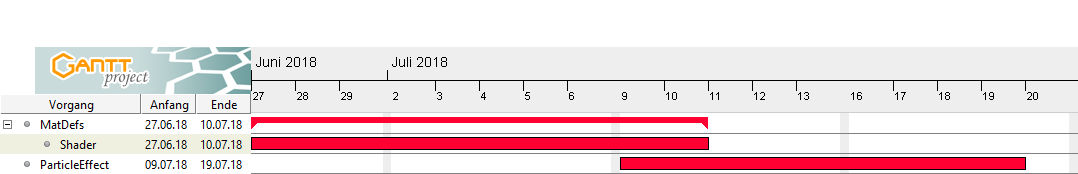
\includegraphics[width=\linewidth]{./Bilder/GanttJonas.png}
		\caption{Jonas - Gantt - Diagramm}
	\end{figure}
	\begin{figure}[htbp]
		\centering
		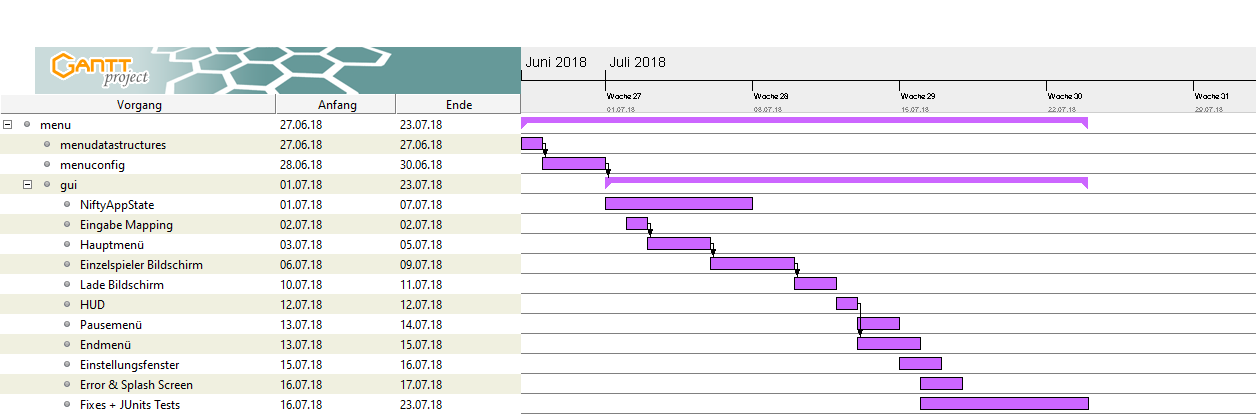
\includegraphics[width=\linewidth]{./Bilder/GanttArtur.png}
		\caption{Artur - Gantt - Diagramm}
	\end{figure}
	\begin{figure}[htbp]
		\centering
		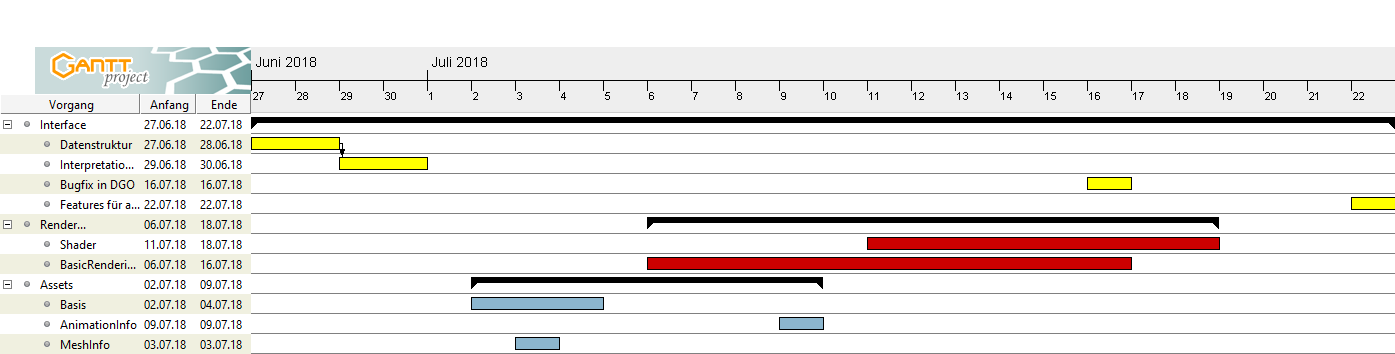
\includegraphics[width=\linewidth]{./Bilder/GanttFrederik.png}
		\caption{Frederik - Gantt - Diagramm}
	\end{figure}
	\begin{figure}[htbp]
		\centering
		\includegraphics[width=\linewidth]{./Bilder/Gantt_Generierung.png}
		\caption{Lukas und Sidney - Gantt - Diagramm}
	\end{figure}

\end{document}